\documentclass[25pt,a1paper]{tikzposter}

%% Tikzposter is highly customizable: please see
%% https://bitbucket.org/surmann/tikzposter/downloads/styleguide.pdf

%% Available themes: see also
%% https://bitbucket.org/surmann/tikzposter/downloads/themes.pdf
% \usetheme{Default}
% \usetheme{Rays}
% \usetheme{Basic}
% \usetheme{Simple}
\usetheme{Envelope}
% \usetheme{Wave}
% \usetheme{Board}
% \usetheme{Autumn}
% \usetheme{Desert}

%% Further changes to the title etc is possible
% \usetitlestyle{Default}
% \usetitlestyle{Basic}
% \usetitlestyle{Empty}
% \usetitlestyle{Filled}
% \usetitlestyle{Envelope}
% \usetitlestyle{Wave}
% \usetitlestyle{verticalShading}

\usepackage{fontspec}
\setmainfont{FreeSerif}
\setsansfont{FreeSans}

\title{HEALTHY ADULTS NEEDED}
\author{Are you between the ages of 18-30 or 60-80 years?}
\institute{Interested in helping out with research?}
%% Optional title graphic
\titlegraphic{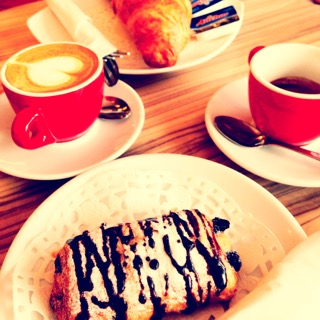
\includegraphics[width=7cm]{IMG_1934}}
%% Uncomment to switch off tikzposter footer
\tikzposterlatexaffectionproofoff

\begin{document}
\maketitle

\block{What is the purpose of this study?}{
\begin{itemize}
\item Develop tasks to detect changes in mood, memory and motivation across lifespan
\item Better
\end{itemize}
}

% \note[rotate=8, connection, width = 7cm,
% % roundedcorners=15, targetoffsetx=2cm
% ]{Oh wait! A note!}

\begin{columns}

\column{0.7}
\block{A test!}{
\begin{itemize}
\item We try to do this. what?
\item we try to do that.
\end{itemize}
}

\column{0.3}
\block{A test!}{
\begin{itemize}
\item We try to do this. what?
\item we try to do that.
\end{itemize}
}

\end{columns}

\block{Random Picture}{%
\begin{tikzfigure}[Figures in tikzposter]
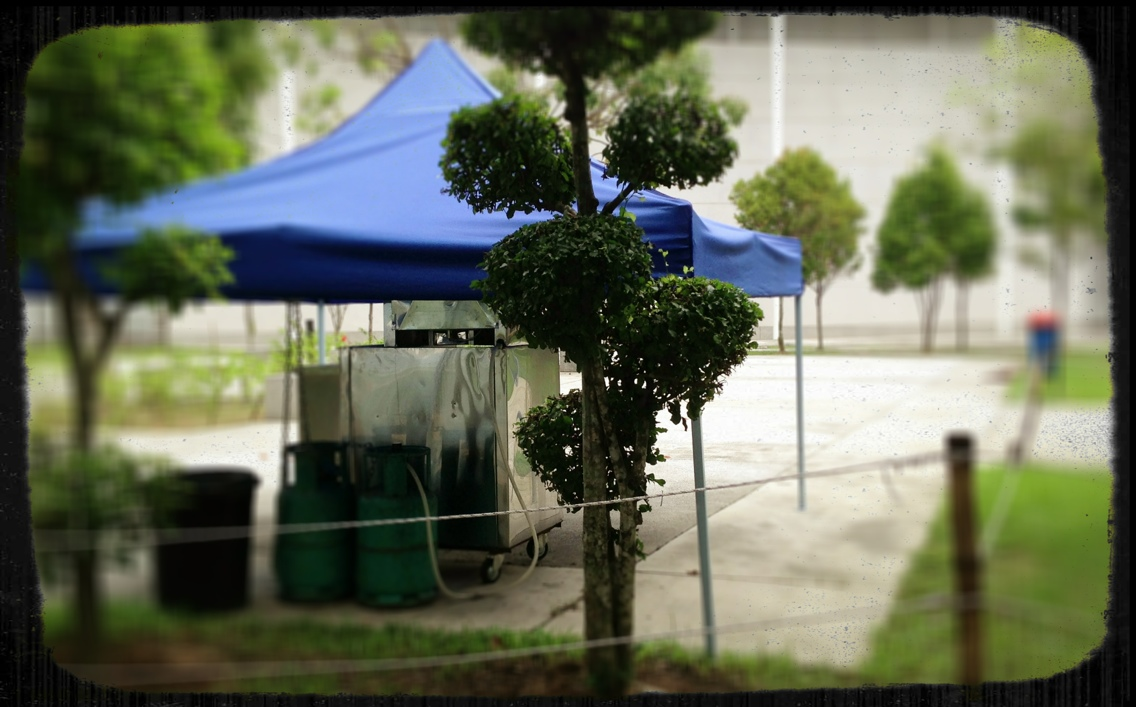
\includegraphics[width=\linewidth]{Photo_4}
\end{tikzfigure}
}

\end{document}